
\chapter{Présentation de l'entreprise}

\section{Smile}

Fondé en 1991, Smile est devenu dès 1995 un acteur du web réputé, maîtrisant l’architecture, les techniques et les outils qui permettent de construire les plus grandes plateformes de l’Internet.
Depuis 2001, Smile est intégrateur de solutions open source, c'est-à-dire que le cœur de métier de Smile est la construction de systèmes d’informations et de plateformes web intégrant les meilleures solutions open source du marché.
Smile mène une forte action de veille afin d’identifier les solutions open sources les plus matures et les plus pérennes, qui apporteront un réel bénéfice de compétitivité pour les entreprises. Smile met à disposition un échantillon de cette expertise au travers de livres blancs, librement diffusés, qui sont devenus des références dans leurs domaines.
Premier intégrateur spécialisé sur les solutions open source, Smile a été choisi à de nombreuses reprises par les plus grandes entreprises et administrations pour déployer ces solutions dans le cadre de projets stratégiques.
Autour du cœur de métier qu’est l’ingénierie, Smile propose une palette de services étendus, qui lui permet de prendre en charge un projet dans sa globalité : consulting en amont et en accompagnement des projets, agence interactive intervenant tant en création et web design où’en conseils éditoriaux, stratégiques et e-marketing, tierce-maintenance applicative (TMA), formation, support et maintien en conditions opérationnelles, et enfin hébergement et exploitation.
Smile possède également un rayonnement international grâce à ses dix-sept agences réparties dans 9 pays.

\begin{figure}[!h]
  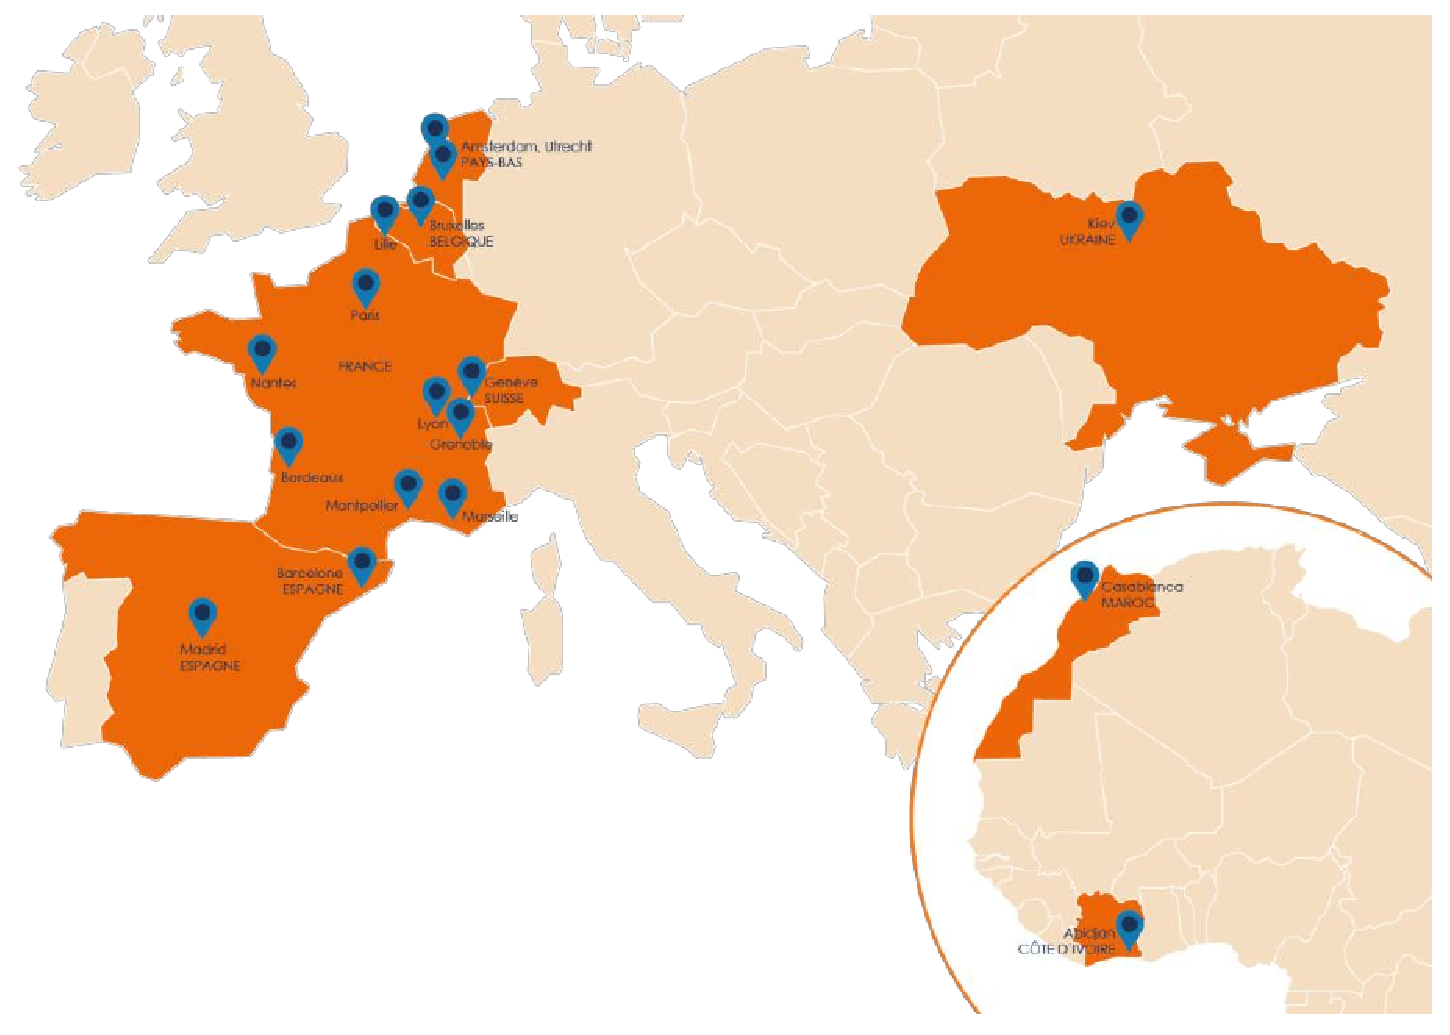
\includegraphics[scale=0.7]{carte_smile}
  \caption{\label{smile_map} Agences Smile}
\end{figure}

Smile organise également une veille technologique importante sur l’open source, avec la rédaction de nombreux livres blancs par les différents consultants sur des sujets variés allant des solutions web d’e-commerce, en passant par les middlewares et finissant par l’embarqué. Il existe actuellement une vingtaine de livres blancs, renouvelés tous les 2-3 ans pour inclure les nouveautés des différents techniques.Dès 2001, Smile commence à construire son expertise des solutions open source : un choix d’avenir que beaucoup de ses concurrents n’osent pas alors entreprendre.À partir de 2004, les grandes entreprises adoptent de plus en plus souvent les solutions open source. Smile occupe une position solide de leader sur ce marché qui décolle, élargissant progressivement son offre vers de nouveaux domaines – CMS, Portails, e-Commerce;Décisionnel, Infrastructure, ERP - et créant des services associés : agence média, tierce maintenance, exploitation, système.  En 2007, Smile affiche plus de 50\% de croissance et inaugure trois nouvelles agences à Lyon, Nantes et Bordeaux.En 2008, Smile compte plus de 270 collaborateurs et poursuit sa croissance en se développant à l'international, notamment à Kiev en Ukraine.En 2009, Smile compte 320 collaborateurs dans le monde et poursuit son extension internationale. En juin 2009, Smile intègre Cometa Technologies S.L., basée à Barcelone et compte alors 8 agences dans le monde.En 2011, Smile regroupe 500 collaborateurs et ouvre ses agences à Bruxelles, Utrecht etAmsterdam.
En 2013, Smile compte 700 collaborateurs et 17 agences.
2014 est une année importante pour Smile, avec plus de 20\% de croissance sur ces cinq
dernières années et près de 700 collaborateurs dans le monde. Au fil de ces années, Smile est
devenu un acteur incontournable de l’open source, leader en France et en Europe.
En 2015, Smile annonce être en négociations exclusives avec la société Open Wide en vue
d’un rapprochement. Ceci afin d'élargir son offre et renforcer son leadership.


\section{Smile ECS}
Smile ECS, ex-Openwide est une société spécialisée dans le domaine de l'open source, racheté par Smile. J'ai décidé d'intégrer cette entreprise pour mon projet de fin d'études à l'université Paris 8 afin d'approfondir mes connaissances dans le domaine du logiciel libre, et celui de l'embarqué. Les techniques Open source devenant de plus en plus prédominants dans le paysage informatique moderne, intégrer une société spécialisée dans cette technique était une façon pour moi de donner un cap sur l'orientation de ma carrière professionnelle.Ce rapport explicitera mon travail durant ce stage de fin d'études, qui a duré six mois, dont le sujet a été d'améliorer le système de transmission des données, afin de pouvoir transmettre un flux vidéo, de caméras de sécurité, avec des métadonnées calculées depuis ce flux (exemple: positions des visages détectés). Puis dans un second temps, récupérer ce flux afin de le stocker pour un visionnage ultérieur.Après une explication du cadre du stage, j'essaierai de développer les techniques utilisés lors de ce stage.